% !TeX root = proyecto.tex

%=========================================================
\chapter{MARCO TEÓRICO}
\setcounter{figure}{0}
En este capítulo se establecerán los fundamentos teóricos sobre los cuales se diseñará la solución para satisfacer las necesidades de las cafeterías universitarias. Se abordará la usabilidad del software, las arquitecturas usadas para sistemas similares y algoritmos de priorización. 

\section{PRINCIPIOS DE USABILIDAD}
Con anterioridad se discutieron las aportaciones Shneiderman y Plaisant \cite{shneiderman2005designing} sobre la usabilidad y las reglas que establecieron, es por ello por lo que se profundizará en esas reglas denominadas las 8 reglas de oro de la usabilidad.
\begin{enumerate}
    \item \textbf{Esforzarse por la consistencia}. Aunque es la regla que más se omite, se sugiere mantener secuencias de acción y componentes consistentes, terminología idéntica en las pantallas y emplear colores, diseños, fuentes y tipografía uniformes en todo el sistema. 
    \item \textbf{Atender la usabilidad universal}. Se debe considerar la diversidad física y cultural de los usuarios que interactuarán con el sistema.
    \item \textbf{Ofrecer retroalimentación informativa}. Por cada acción que realice el usuario, el sistema debe responder en función de la frecuencia de las acciones en el proceso, evitando saturar de información a los involucrados en acciones y procesos más usados.
    \item \textbf{Diseñar diálogos que generan cierre}. Agrupar las secuencias de acción y dar un sentido de inicio, desarrollo y cierre para promover la satisfacción y alivio de haber cumplido la tarea. 
    \item \textbf{Prevenir errores}. El sistema debe limitar las acciones del usuario si estas comprometen la integridad del proceso y, en caso de que ocurran, proporcionarle al usuario información del error y proponer soluciones. 
    \item \textbf{Permitir la reversión sencilla de acciones}. Si las acciones se pueden deshacer, le proporcionan al usuario la tranquilidad de poder experimentar y familiarizarse con el software sin temor a consecuencias irreversibles.
    \item \textbf{Apoyar el locus de control interno}. El sistema debe responder a las acciones del usuario. Diseñar interfaces que provoquen el efecto contrario ocasionará falta de confianza en el software.
    \item \textbf{Reducir la carga de la memoria a corto plazo}. Condensar procesos en la menor cantidad de pantallas posibles (asegurando la alineación con las reglas anteriores) le proporciona al usuario el tiempo de respuesta necesario para mantener noción de sus acciones, reduciendo la carga cognitiva y la saturación visual. 
\end{enumerate}

Considerando la teoría anterior, si el sistema busca la satisfacción del flujo de trabajo a la par de la evocación de sentimientos satisfactorios, tendrá más éxito en su integración; especialmente en aquellos entornos donde la cultura desconfía de la novedad. 

Es por esto por lo que, bajo los principios de Shneiderman y Plaisant \cite{shneiderman2005designing}, se estructurará el diseño de las interfaces de usuario de la solución propuesta para apegarse a estas reglas, con el objetivo de facilitar la integración del software en el entorno de las cafeterías de las unidades académicas que se caracteriza por ser ruidoso, con pocas oportunidades de precisión mecánica y donde el contraste visual es relevante para distinguir objetos y botones en una pantalla.

\section{TRANSFORMACIÓN DIGITAL EN LA INDUSTRIA GASTRONÓMICA}
La transformación digital en el sector de servicios alimentarios se define como la integración de tecnologías de la información y comunicación para optimizar la productividad y la experiencia del cliente. Este fenómeno impacta tanto en las operaciones de \textit{Front-of-House} (FoH), mediante tecnologías que asisten los procesos del cliente, como en el \textit{Back-of-House} (BoH), donde se busca agilizar las tareas administrativas y de cocina y Lee et al. \cite{woojin2024effect}\cite{woojin2026multifaceted} mencionan estos términos para explicar el impacto de la transformación digital. La adopción de estas herramientas permite superar problemas de baja productividad mediante la creación de flujos de trabajo simplificados.

Para el término FoH establecen que comprende a todos los espacios físicos y digitales de interacción directa con el cliente, capturando acciones como la toma de pedidos, procesamiento de pagos y la gestión de reseñas. Mientras que para el término complementario BoH se establecen todas las operaciones que el cliente no interactúa directamente y que están centradas en la producción y la administración, como por ejemplo la preparación de alimentos, la gestión de inventario, la cadena de suministro y la programación de turnos laborales. 

Lee et al. destacan que la tecnología en ambos ámbitos cumple dos funciones: una función exploradora en la que permite usar datos recolectados para innovar en los productos y mejorar los procesos de tomas de decisiones, y una función explotadora en la que optimiza los recursos disponibles para brindar estabilidad operativa durante horas de alta demanda. 

Bajo estas definiciones de Lee et al. \cite{woojin2026multifaceted} se dividirán los módulos del sistema para mantener las funciones con divisiones operativas claras. 

\section{ARQUITECTURA DEL KMS}
En el estudio de Nwekori e Ignatius \cite{nwekori2025design} se propone una arquitectura como la de la Imagen \ref{fig:arquitecturaNwekoriIgnatius}, donde el sistema está descentralizado con respecto a la base de datos, pero mantiene una separación de interfaces clara para interactuar con el cliente y con el personal de la cafetería. A su vez, mantiene 4 módulos funcionales entre las interfaces: el módulo de registro y autenticación de usuario, el módulo de gestión de menú, el módulo de gestión de órdenes y el módulo de integración de pasarela de pagos.

\begin{figure}[htbp]
    \begin{center}
        \fbox{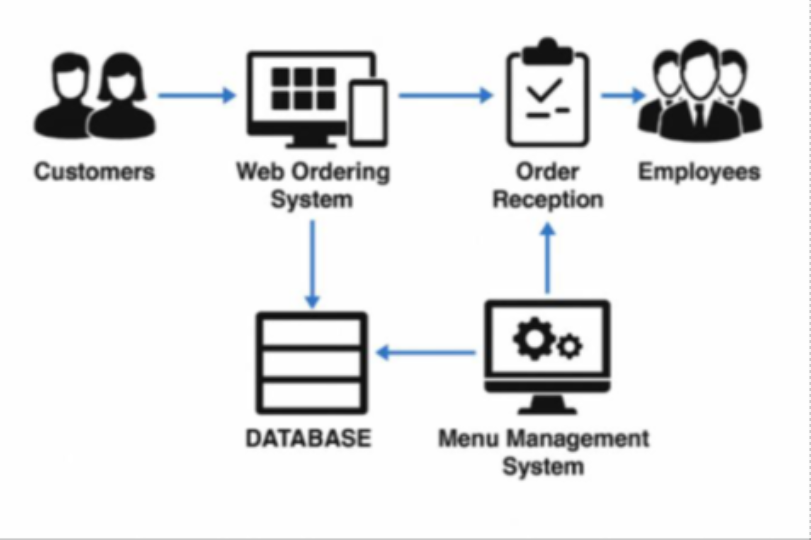
\includegraphics[width=.8\textwidth]{cdt/images/Arquitectura_Nwekori-Ignatius}}
        \caption{Arquitectura del sistema de Nwekori e Ignatius \cite{nwekori2025design}.}
        \label{fig:arquitecturaNwekoriIgnatius}
    \end{center}
\end{figure}
